\documentclass[conference]{IEEEtran}
\IEEEoverridecommandlockouts

\usepackage{cite}
\usepackage{amsmath,amssymb,amsfonts}
\usepackage{algorithmic}
\usepackage{graphicx}
\usepackage{textcomp}
\usepackage{xcolor}
\usepackage{booktabs}
\usepackage{array}
\usepackage{multirow}
\def\BibTeX{{\rm B\kern-.05em{\sc i\kern-.025em b}\kern-.08em
    T\kern-.1667em\lower.7ex\hbox{E}\kern-.125emX}}
\begin{document}

\title{Enhanced Multi-Authority Ethical Supply Chain Tracking System Using Blockchain for Transparent Healthcare Verification}

\author{\IEEEauthorblockN{Suyash Jain}
\IEEEauthorblockA{\textit{Department of Networking and Communications} \\
\textit{SRM Institute of Science and Technology}\\
Kattankulathur, India \\
sj5889@srmist.edu.in}
\and
\IEEEauthorblockN{Prince Bagla}
\IEEEauthorblockA{\textit{Department of Networking and Communications} \\
\textit{SRM Institute of Science and Technology}\\
Kattankulathur, India \\
pb0795@srmist.edu.in}
\and
\IEEEauthorblockN{Godwin J Ponsam}
\IEEEauthorblockA{\textit{Department of Networking and Communications} \\
\textit{SRM Institute of Science and Technology}\\
Kattankulathur, India \\
godwinj@srmist.edu.in}
}

\maketitle

\begin{abstract}
This paper presents an improved blockchain-based supply chain tracking system for healthcare. The key new feature is a voting-based approval system where at least 2 out of 3 registered authorities must approve a product before it can move forward in the supply chain. This solves a major problem in older systems --- any single person could push a product through the chain with no checks at all. We built and tested the system on the Sepolia Ethereum test network. Compared to the older system, our system uses 47\% less gas (transaction cost) for registering a product. We also added role-based access control so each user can only do what their role allows, a blacklist to block bad actors, and a feature to stop duplicate votes. We tested the system across eight quality measures and found clear improvements in trust, security, governance, validation, and record-keeping. The system gives healthcare supply chains a simple, transparent, and tamper-proof way to verify products before they reach patients.
\end{abstract}

\begin{IEEEkeywords}
Blockchain, supply chain management, healthcare verification, smart contracts, multi-authority validation, threshold-based governance, Ethereum, IPFS.
\end{IEEEkeywords}

\section{Introduction}

The healthcare supply chain is the process of making, moving, and delivering medicines and medical devices to patients. According to the World Health Organization, around 10\% of medicines in developing countries are fake or substandard, which directly harms patients. Large supply networks with many parties involved make it hard to track where a product came from, which opens the door to fake products, contamination, and theft.

Blockchain has been studied as a solution to this problem. It works like a shared digital record book that nobody can change. Because there is no single central owner, it is harder to cheat the system. In healthcare, blockchain has been used to track medicine batches, check supplier details, and keep permanent audit records.

Latif et al. built a blockchain-based medicine supply chain system that tracks a product from creation all the way to the patient \cite{b1}. It showed that smart contracts --- self-running programs on the blockchain --- can automatically enforce supply chain rules. However, that system has one big problem: a single person owns each product at any time and can pass it to anyone else with no checks. There is no authority reviewing whether the product is safe or legal, and there is no way to stop the contract in an emergency.

This paper proposes an improved system that adds a mandatory approval checkpoint. Before a product can be distributed, it must be reviewed and approved by multiple independent authorities. Only when enough authorities agree does the product move forward. We built, deployed, and tested this system, then compared it against the older model on cost, security, and features.

\section{Literature Review}

Blockchain for supply chains has been an active research area since the mid-2010s. It started with digital payments but grew into a tool for tracking products through complex networks using smart contracts.

Latif et al. built the baseline medicine supply chain system we improve upon in this paper \cite{b1}. Their system tracks a product through six steps: created, for sale, sold, shipped, received, and consumed. At each step, the current owner passes the product to the next person. The full history of who owned the product is stored on the blockchain and can be checked at any time. This proved that smart contracts can run supply chain rules automatically.

Blockchain has also been used outside healthcare --- for tracking food, luxury items, and car parts \cite{b2}, \cite{b3}. These systems all follow the same basic pattern: a smart contract handles the rules, the blockchain stores the records, and users interact through a web app with a crypto wallet. Healthcare needs more than this basic pattern because it also requires regulatory checks, document verification, and approval from multiple parties.

Storing documents directly on the blockchain is very expensive. A better approach is to store documents on IPFS --- a decentralized file system --- and only store a short fingerprint (hash) of the document on-chain \cite{b7}. This way, the document can be verified without paying high storage costs. This method is used in systems for medical records and academic certificates.

The idea of needing a minimum number of approvers before something is accepted comes from distributed computing research. It has been used in blockchain consensus systems but applying it inside a supply chain smart contract as an ethical approval gate is a newer idea that this paper explores.

\section{Research Gap and Motivation}

We studied the baseline system by Latif et al. and found four clear problems that make it unsuitable for real healthcare use.

\subsection{Single-Owner Authorization}

In the baseline system, one person owns each product and can pass it to anyone else with no outside check. If that person is dishonest or makes a mistake, a fake or unsafe product can move through the entire supply chain without anyone catching it.

\subsection{Absence of Validation Gates}

The baseline has no checkpoint where a product's certificates or quality documents are checked. Once a product is created, it can flow all the way to the patient without any authority ever reviewing it.

\subsection{Limited Governance Controls}

The baseline has no way to ban a bad actor from the system, pause the contract if something goes wrong, or remove a user's permissions. In a real healthcare network, these controls are necessary for managing security problems and policy violations.

\subsection{No Certificate Verification}

Healthcare products must come with documents proving they meet quality and safety standards. The baseline system has no way to attach, store, or check these documents. There is no connection between the product record on the blockchain and the real-world paperwork that proves the product is legitimate.

These four problems motivated us to build an improved system that keeps the tracking strengths of the original while adding the safety checks that real healthcare use requires.

\section{Proposed System Architecture}

Our system is built in five layers, each handling a different part of the work.

\textbf{Layer 1 --- User Layer.} The people who use the system are: the admin, the manufacturer, the regulatory authority, the distributor, the retailer, and the public verifier. Each person can only do things that match their role.

\textbf{Layer 2 --- Frontend Layer.} The website is built using Next.js, TypeScript, and Tailwind CSS. It has two main pages. The home page lets users interact with the contracts based on their role. The verification page lets anyone look up a product and generate a QR code for it.

\textbf{Layer 3 --- Wallet Layer.} Users connect their MetaMask wallet to the website. MetaMask signs and sends transactions to the Ethereum network. The Ethers.js library handles the connection between the website and the blockchain.

\textbf{Layer 4 --- Blockchain Layer.} Two smart contracts are deployed on the Sepolia test network. The first is the original baseline contract, kept for comparison. The second is our new improved contract with the approval voting system, role controls, and emergency features. Both run on the same network so we can compare them fairly.

\textbf{Layer 5 --- Off-Chain Storage Layer.} Compliance certificates are uploaded to IPFS through the Filebase service. Filebase returns a unique file ID (called a CID). We convert that ID into a short hash and store it in the product record on the blockchain. This links the product to its certificate without storing the whole document on-chain, keeping costs low.

\begin{figure}[htbp]
\centerline{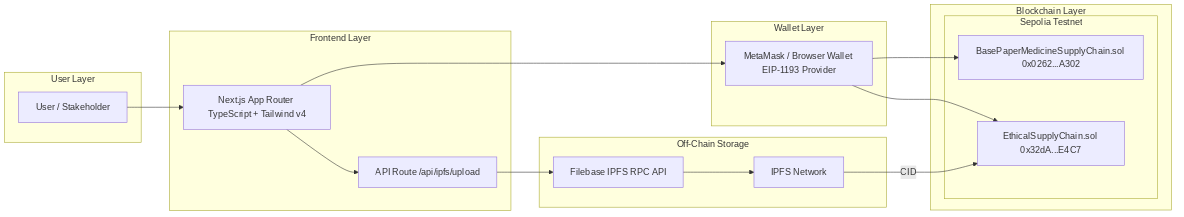
\includegraphics[width=\columnwidth]{architecture.png}}
\caption{System architecture showing five-layer design from user through off-chain storage.}
\label{fig:architecture}
\end{figure}

\section{Threshold-Based Algorithm}

The main new feature of our system is the Threshold-Based Multi-Authority Ethical Validation Algorithm. It creates a voting gate that every product must pass before it can be distributed.

\subsection{Algorithm Parameters}

The system requires at least 2 out of 3 registered authorities to approve a product before it can move forward. Three authorities must always be registered for the system to work. The admin can change the required number of approvals, but cannot set it higher than the total number of registered authorities.

\subsection{Algorithm Steps}

The process works as follows. First, a manufacturer registers a product on the blockchain with a product ID, a certificate hash from IPFS, and details like batch number, manufacturer name, and manufacturing and expiry dates. Second, the manufacturer marks the product as ``Manufactured.'' Third, the registered authorities look at the certificate on IPFS and each casts a vote to approve or reject. Fourth, after every vote, the contract checks if enough votes have been cast. Fifth, if approvals reach the threshold, the product is marked ``Approved.'' If rejections reach the threshold, it is marked ``Rejected'' permanently. Sixth, the contract blocks any product from moving past the Manufactured stage unless it is Approved.

\begin{figure}[htbp]
\centerline{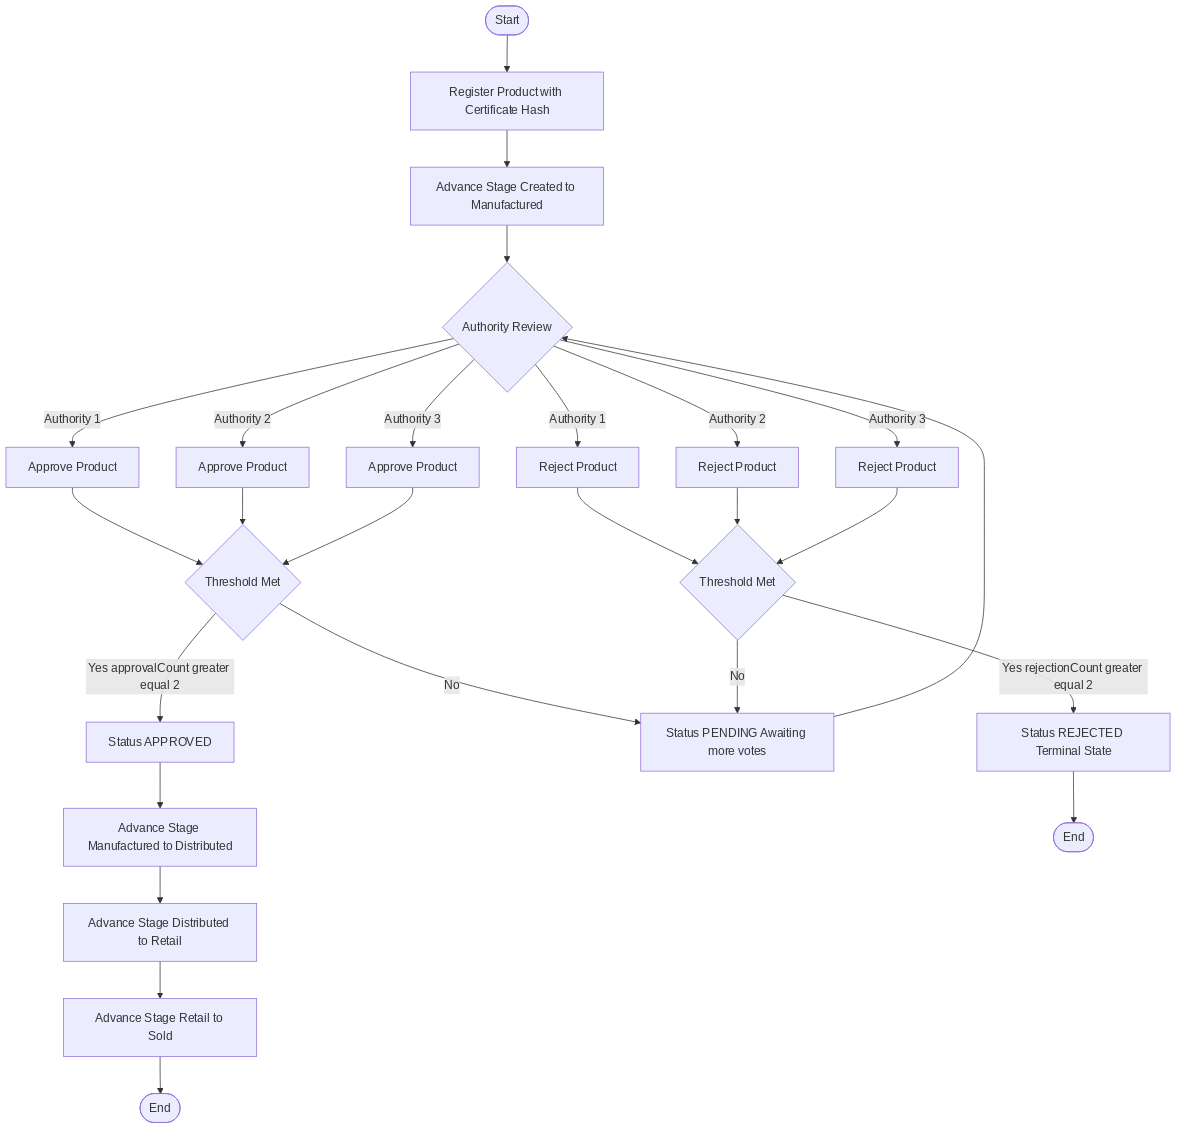
\includegraphics[width=0.85\columnwidth]{flowchart.png}}
\caption{Proposed system flowchart with threshold validation gate and approval/rejection paths.}
\label{fig:flowchart}
\end{figure}

\subsection{Guard Conditions}

The algorithm has eight safety checks built in, listed in Table~\ref{tab:guards}. Each check blocks a specific type of wrong action. If any check fails, the transaction is cancelled and a clear error message is returned.

\begin{table}[htbp]
\caption{Guard Conditions Enforced by the Validation Algorithm}
\label{tab:guards}
\begin{center}
\renewcommand{\arraystretch}{1.1}
\begin{tabular}{|>{\raggedright\arraybackslash}p{2.4cm}|>{\raggedright\arraybackslash}p{2.4cm}|>{\raggedright\arraybackslash}p{2.2cm}|}
\hline
\textbf{Guard} & \textbf{Enforcement Point} & \textbf{Failure Result} \\
\hline
Contract not paused & whenNotPaused modifier & ContractPaused revert \\
\hline
Actor not blacklisted & onlyActiveRole modifier & AccountBlacklisted revert \\
\hline
Correct role for stage & hasRole check & InvalidRoleForStage revert \\
\hline
Current custodian & custodian comparison & NotCurrentCustodian revert \\
\hline
Validation passed & status check at Manufactured & ValidationRequired revert \\
\hline
No duplicate votes & hasValidated mapping & AlreadyValidated revert \\
\hline
Validation still open & Pending status check & ValidationClosed revert \\
\hline
\end{tabular}
\end{center}
\end{table}

\subsection{Approval and Rejection Logic}

After each authority votes, the contract counts the total approvals. If the count reaches the required threshold, the product is marked Approved and can move forward. The same counting logic applies to rejections --- if enough authorities reject, the product is permanently blocked. A rejected product cannot be re-submitted or moved forward under any circumstances.

\subsection{Algorithm Pseudocode}

\begin{algorithmic}
\STATE \textbf{function} registerProduct(productId, certificateHash, metadata)
\STATE \hspace{1em} require(msg.sender has MANUFACTURER\_ROLE)
\STATE \hspace{1em} require(product does not exist)
\STATE \hspace{1em} store Product struct with stage = Created
\STATE \textbf{function} approveProduct(productId)
\STATE \hspace{1em} require(contract not paused)
\STATE \hspace{1em} require(msg.sender has AUTHORITY\_ROLE)
\STATE \hspace{1em} require(!hasValidated[productId][msg.sender])
\STATE \hspace{1em} hasValidated[productId][msg.sender] = true
\STATE \hspace{1em} product.approvalCount++
\STATE \hspace{1em} \textbf{if} product.approvalCount $\geq$ authorityThreshold \textbf{then}
\STATE \hspace{2em} product.validationStatus = Approved
\STATE \textbf{function} advanceStage(productId, nextCustodian)
\STATE \hspace{1em} \textbf{if} currentStage == Manufactured \textbf{then}
\STATE \hspace{2em} require(product.validationStatus == Approved)
\STATE \hspace{1em} product.stage = currentStage + 1
\STATE \hspace{1em} product.currentCustodian = nextCustodian
\end{algorithmic}

\section{Technology Stack}

Table~\ref{tab:stack} lists the tools and technologies used to build the system. Each tool was chosen because it is widely used, well-documented, and works well with the Ethereum ecosystem.

\begin{table}[htbp]
\caption{Technology Stack Used in System Implementation}
\label{tab:stack}
\begin{center}
\renewcommand{\arraystretch}{1.15}
\begin{tabular}{|>{\raggedright\arraybackslash}p{2.8cm}|p{2.4cm}|>{\raggedright\arraybackslash}p{1.8cm}|}
\hline
\textbf{Layer} & \textbf{Technology} & \textbf{Version} \\
\hline
Smart Contract Language & Solidity & 0.8.24 \\
\hline
Contract Framework & Hardhat & 2.24.1 \\
\hline
Security Libraries & OpenZeppelin & v4.9.6 \\
\hline
Frontend Framework & Next.js & 16.2.1 \\
\hline
Frontend Language & TypeScript & 5 \\
\hline
Blockchain Library & Ethers.js & 6.16.0 \\
\hline
Wallet Integration & MetaMask & EIP-1193 \\
\hline
Off-Chain Storage & Filebase IPFS & RPC API \\
\hline
Target Network & Sepolia Testnet & 11155111 \\
\hline
\end{tabular}
\end{center}
\end{table}

The OpenZeppelin library provided three ready-made security modules. AccessControlEnumerable manages the roles and permissions for each user. Pausable lets the admin freeze all contract activity in an emergency. ReentrancyGuard prevents a known attack where a hacker tries to call the contract multiple times in one transaction to drain funds. These three modules form the security backbone of the system.

\section{Implementation and Results}

We fully built and deployed both contracts on the Sepolia test network. Because both contracts run on the same network, we can compare them directly under the same conditions.

\subsection{Working Features}

The baseline contract covers the full six-step product lifecycle from the original paper. The proposed contract covers all of that and adds: approval voting by authorities, role-based access for four actor types, blacklisting of bad actors, emergency pause, duplicate vote prevention, custodian handover checking, next-custodian role checking, manufacturing and expiry date storage, QR code generation for public product lookup, zero-address input checking, reentrancy protection, and compact data storage to save gas.

\subsection{Deployment Details}

The baseline contract is live at address 0x0262C4dEc9A16A5962e862926DD1AdA94c64A302. The proposed contract is live at address 0x32dA54F4c606fccB17fcB3f41416529b181cE4C7. Both are on the Sepolia test network (chain ID 11155111) and can be viewed publicly on the Sepolia block explorer.

\subsection{Gas Consumption Analysis}

Gas is the fee paid for running operations on the Ethereum blockchain. Lower gas means cheaper transactions. We measured gas usage for three common operations on both contracts under the same conditions. Our system saves gas mainly because we use small data types: numbers stored as uint8 (1 byte) instead of strings, and timestamps stored as uint32 instead of uint256. This means less data is written to the blockchain per transaction.

\begin{table}[htbp]
\caption{Gas Consumption Comparison Across Three Operations}
\label{tab:gas}
\begin{center}
\renewcommand{\arraystretch}{1.2}
\begin{tabular}{|>{\raggedright\arraybackslash}p{2.6cm}|c|c|c|}
\hline
\textbf{Operation} & \textbf{Baseline} & \textbf{Proposed} & \textbf{Savings} \\
\hline
Create / Register & 145,056 & 76,085 & 47.6\% \\
\hline
Sell / Advance Stage & 76,558 & 38,450 & 49.8\% \\
\hline
Buy / Approve & 81,291 & 59,786 & 26.5\% \\
\hline
\end{tabular}
\end{center}
\end{table}

Registering a product costs 47.6\% less gas in our system. Moving a product to the next stage costs 49.8\% less. The approval operation saves only 26.5\% because it does extra work --- counting votes and checking the threshold --- that the baseline does not do at all.

\begin{figure}[htbp]
\centerline{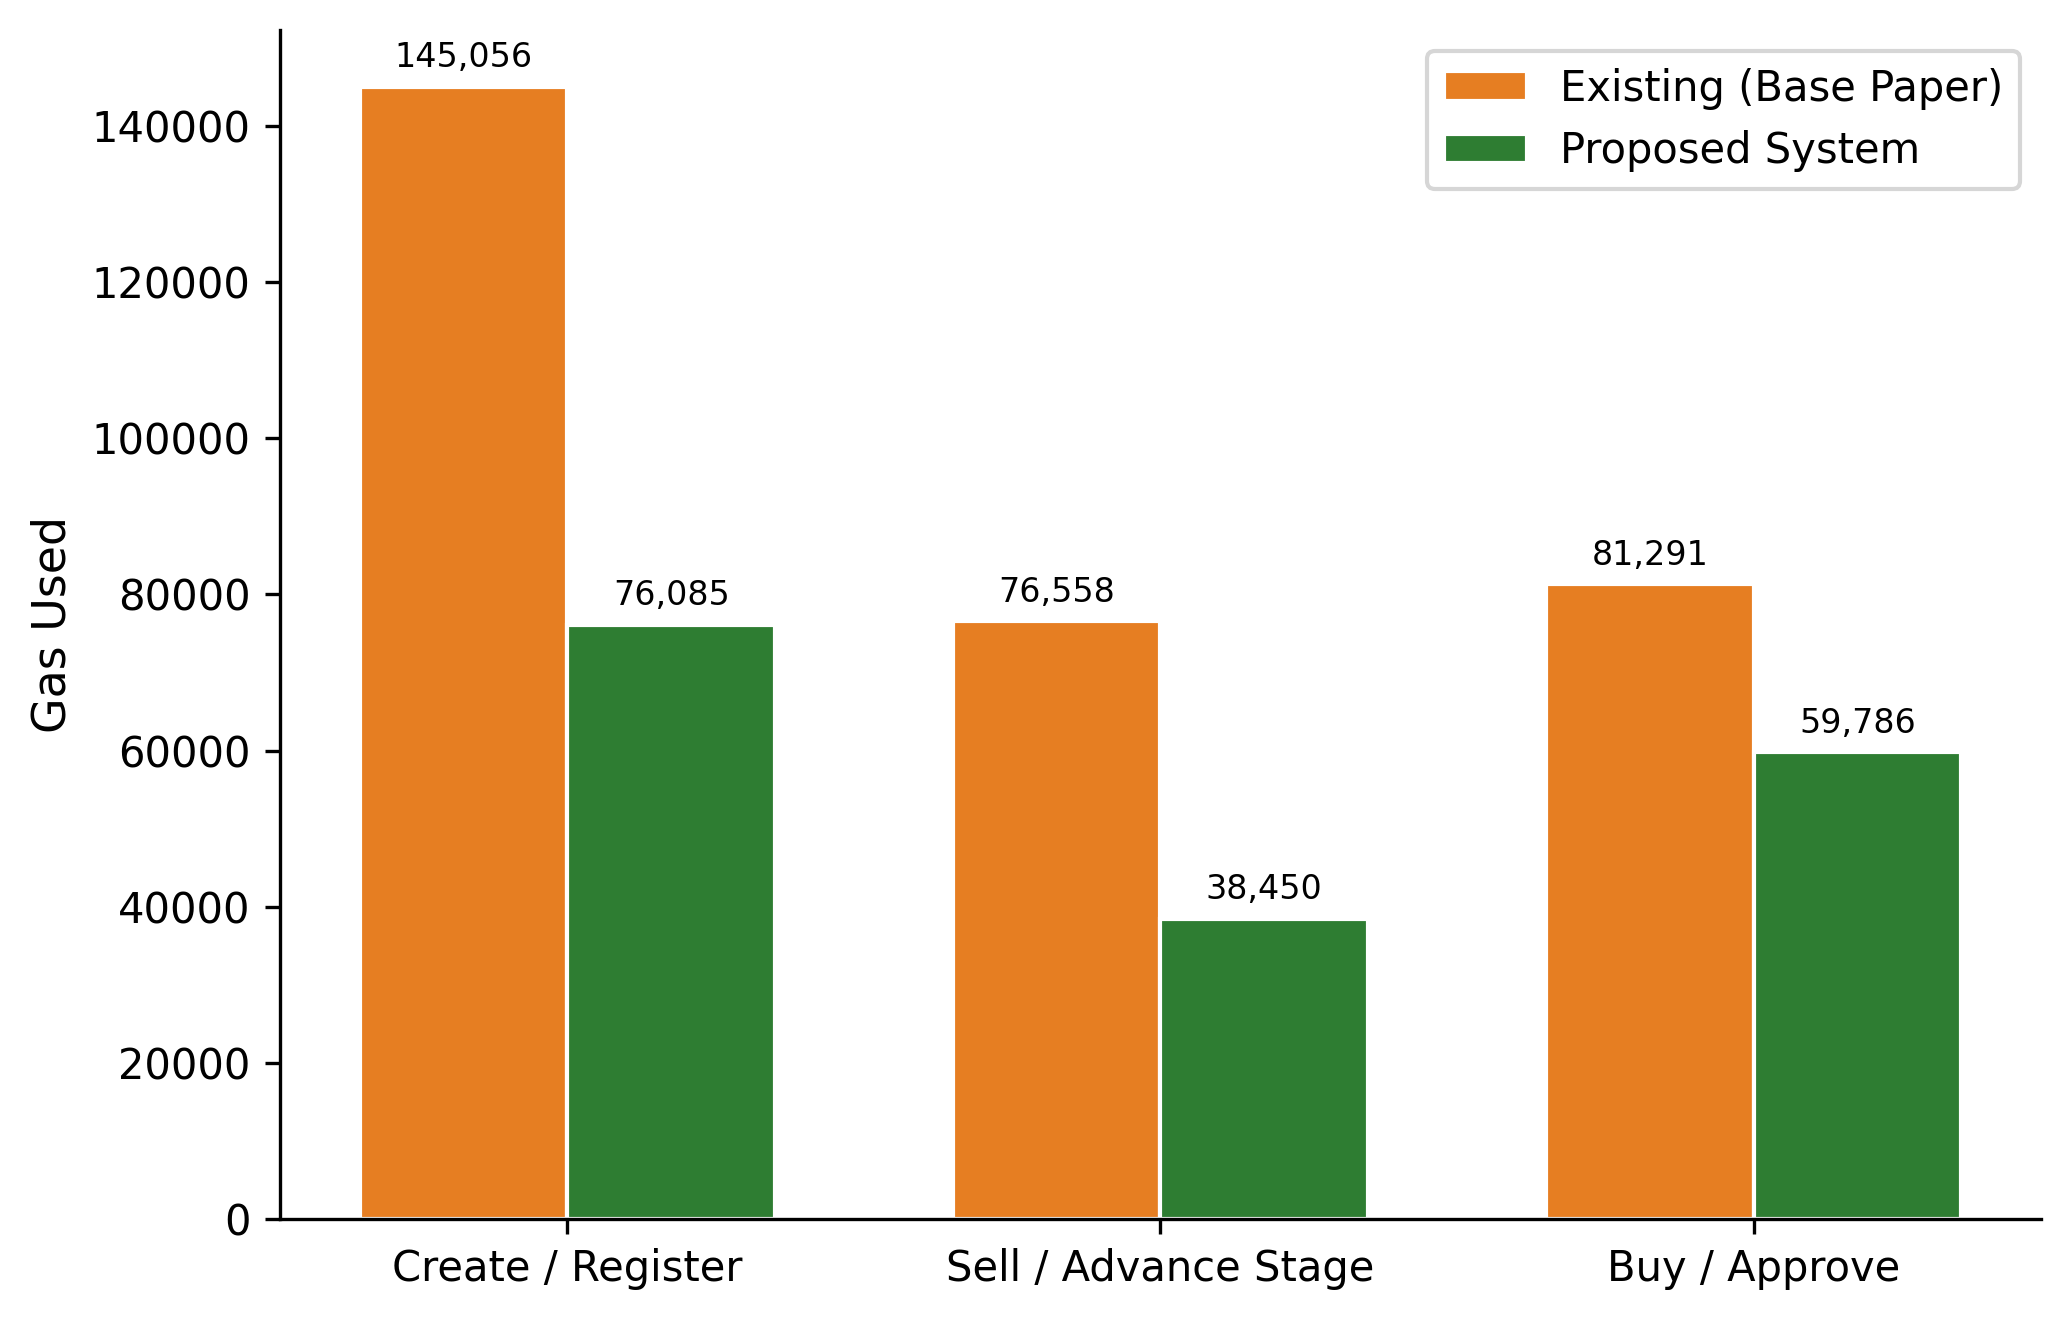
\includegraphics[width=\columnwidth]{bar_chart.png}}
\caption{Gas usage comparison across three operations between baseline and proposed systems.}
\label{fig:barchart}
\end{figure}

\section{Comparative Analysis}

We compared both systems across eight quality areas. Each area was scored out of 10 based on what features are present and how well they work.

\subsection{Multi-Dimensional Evaluation}

\textbf{Trust} measures how well the system stops one person from making decisions alone. The baseline scores 4 because any single owner can pass a product to anyone. Our system scores 9 because multiple independent authorities must agree before a product moves forward.

\textbf{Security} covers access controls, input checks, and protection against attacks. The baseline scores 5 with only basic ownership checks. Our system scores 9 by adding role-based access, blacklisting, emergency pause, reentrancy protection, and zero-address checks.

\textbf{Governance} measures what tools admins have to manage the system. The baseline scores 3 --- it has almost no admin controls. Our system scores 9 with a full admin panel for managing roles, setting thresholds, blacklisting users, and pausing the contract.

\textbf{Transparency} measures how visible the product history and decisions are. Both systems keep records on-chain, but our system also records every vote, certificate link, and status change, improving from 7 to 9.

\textbf{Validation} is the biggest difference between the two systems. The baseline scores 2 because there is no approval gate at all. Our system scores 9 because every product must be approved by at least 2 independent authorities before it can be distributed.

\textbf{Storage Efficiency} measures how compactly data is stored on-chain. The baseline uses strings and large 256-bit numbers, scoring 5. Our system uses small data types and packed structs, scoring 8.

\textbf{Gas Efficiency} measures how cheap transactions are. The baseline's create operation costs 145,056 gas versus our 76,085. However, our system adds voting operations the baseline does not have. Overall scores are 5 for baseline and 7 for our system.

\textbf{Auditability} measures how complete the on-chain records are for review. The baseline emits basic events, scoring 6. Our system emits detailed events for every action including votes, rejections, blacklist changes, and threshold updates, scoring 9.

\begin{figure}[htbp]
\centerline{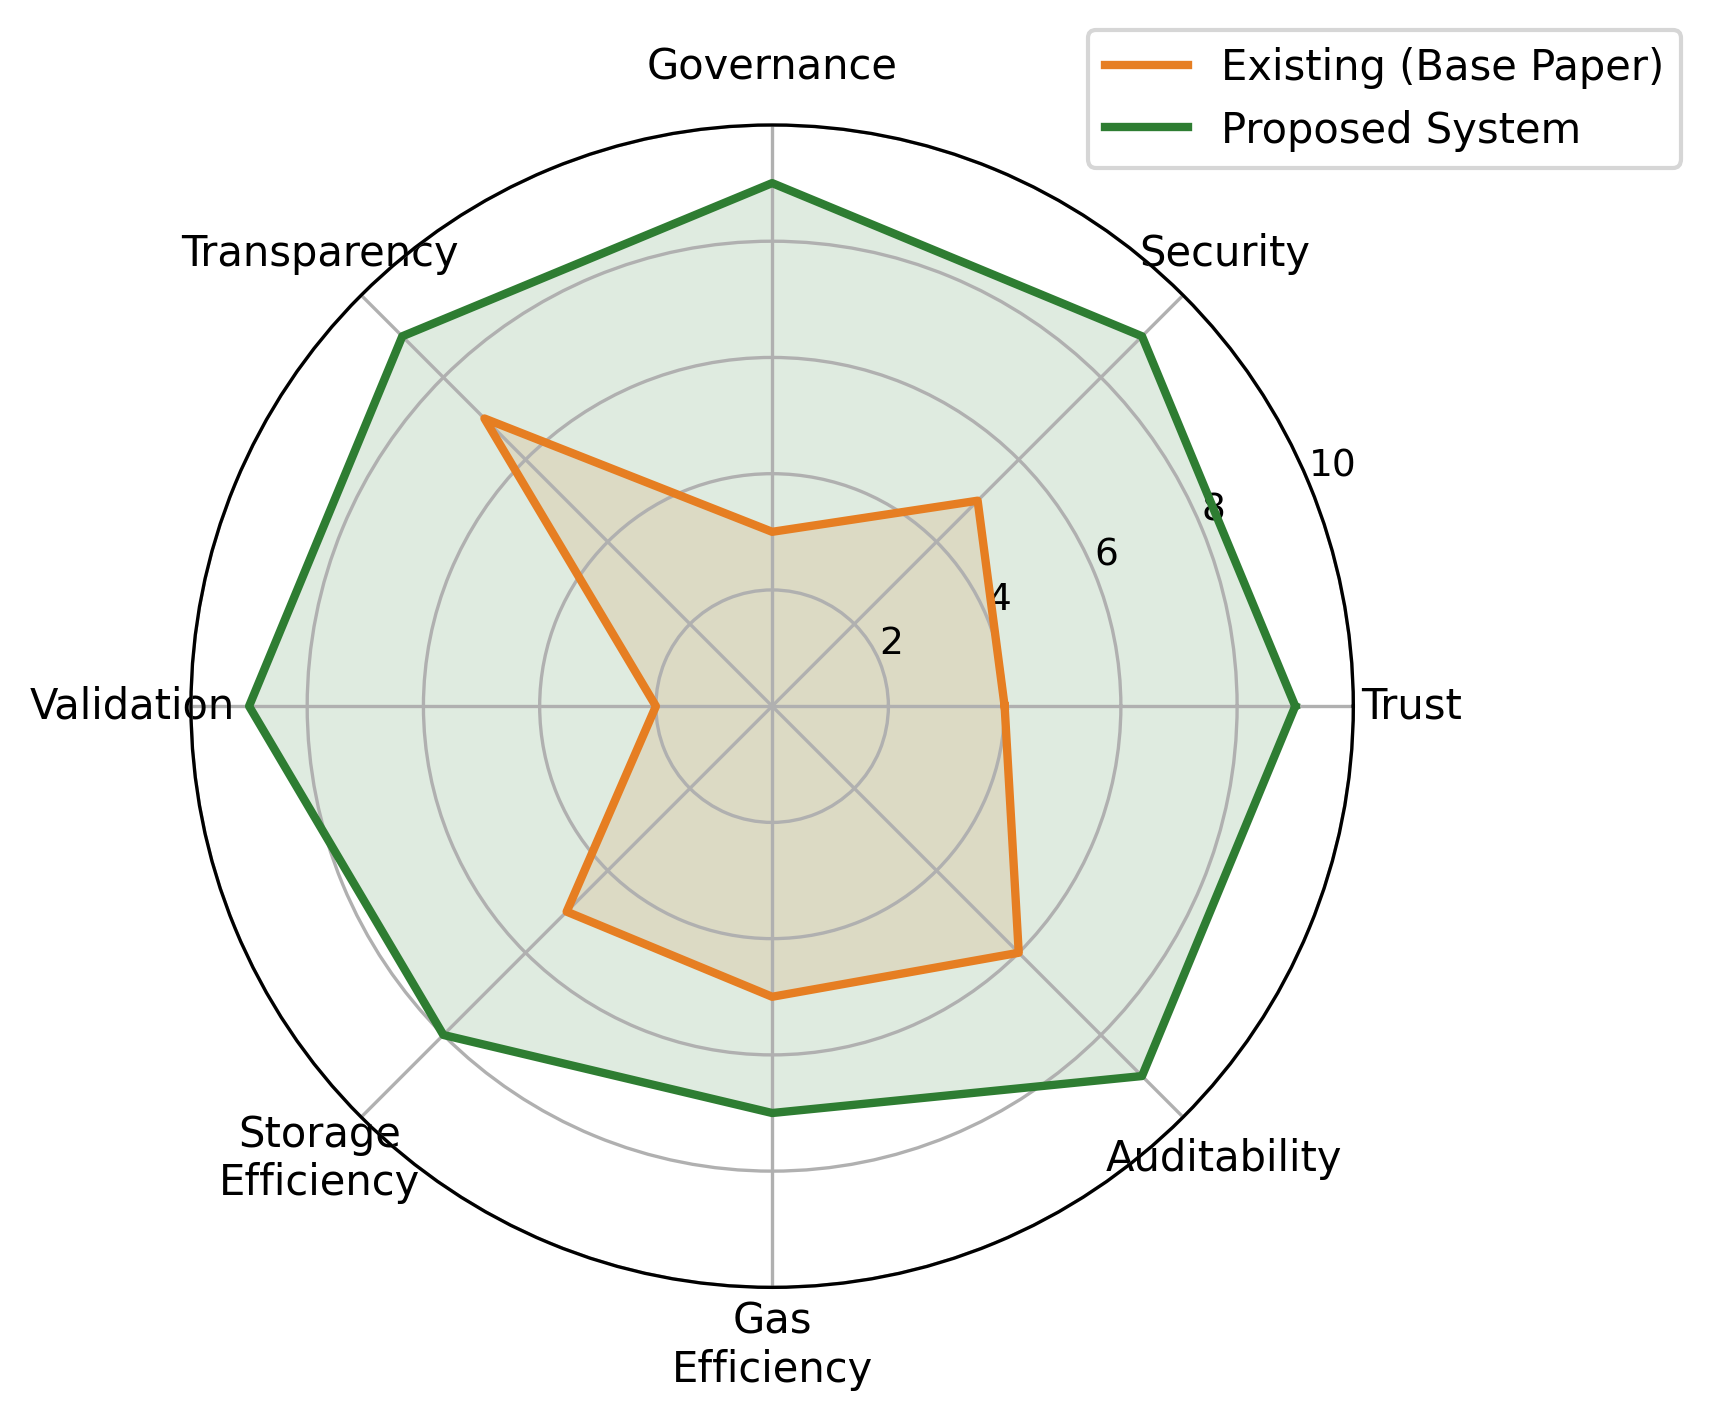
\includegraphics[width=0.9\columnwidth]{radar_chart.png}}
\caption{Eight-dimensional comparison between existing baseline and proposed systems (scale 0--10).}
\label{fig:radar}
\end{figure}

\subsection{Feature Comparison}

Table~\ref{tab:features} shows a direct side-by-side list of features. Our system adds thirteen features that are completely absent from the baseline.

\begin{table}[htbp]
\caption{Feature Comparison Between Baseline and Proposed Systems}
\label{tab:features}
\begin{center}
\renewcommand{\arraystretch}{1.15}
\begin{tabular}{|>{\raggedright\arraybackslash}p{4.8cm}|c|c|}
\hline
\textbf{Feature} & \textbf{Baseline} & \textbf{Proposed} \\
\hline
Multi-authority validation & No & Yes \\
\hline
Certificate verification & No & Yes \\
\hline
Blacklist enforcement & No & Yes \\
\hline
Emergency pause & No & Yes \\
\hline
Role revocation safety & No & Yes \\
\hline
Duplicate vote prevention & No & Yes \\
\hline
Custodian validation & No & Yes \\
\hline
Next-custodian role check & No & Yes \\
\hline
MFG/EXP date tracking & No & Yes \\
\hline
Public QR verification & No & Yes \\
\hline
Zero-address guards & No & Yes \\
\hline
Reentrancy protection & Partial & Yes \\
\hline
Compact storage & No & Yes \\
\hline
\end{tabular}
\end{center}
\end{table}

\section{Conclusion and Future Work}

This paper built and tested an improved blockchain supply chain system for healthcare. The main new idea is a voting gate where at least 2 out of 3 authorities must approve a product before it can be distributed. This directly fixes the biggest weakness in the original system --- that any single actor could move any product through the chain with no oversight.

The system was deployed live on the Sepolia test network. Gas costs dropped by 47.6\% for registration and 49.8\% for stage advancement compared to the baseline. The system also added role-based access control, blacklisting, emergency pause, duplicate vote prevention, certificate storage via IPFS, and detailed on-chain audit events --- all features completely absent from the baseline.

Future work includes adding camera-based QR scanning for field verification, building a role-specific dashboard for easier management, verifying the contracts publicly on Etherscan for third-party audit, and extending the system to support other regulatory frameworks and other blockchain networks beyond Ethereum.

This work shows that a healthcare blockchain supply chain can be made significantly safer and more trustworthy by adding multi-authority governance, without making it more expensive to run.

\section*{Acknowledgment}

The authors acknowledge the Department of Networking and Communications at SRM Institute of Science and Technology, Kattankulathur, for providing the research infrastructure and computational resources used in this work.

\begin{thebibliography}{00}
\bibitem{b1} S. Adarsh, S. G. Joseph, F. John, M. Lekshmi, and S. Asharaf, ``A transparent and traceable coverage analysis model for vaccine supply-chain using blockchain technology,'' \textit{IT Prof.}, vol. 23, no. 4, pp. 28--35, 2021.
\bibitem{b2} U. Agarwal, V. Rishiwal, S. Tanwar, R. Chaudhary, G. Sharma, P. N. Bokoro, and R. Sharma, ``Blockchain technology for secure supply chain management: A comprehensive review,'' \textit{IEEE Access}, vol. 10, pp. 85\,493--85\,517, 2022.
\bibitem{b3} A. Ahmad, N. Verma, N. Sarhan, E. M. Awwad, A. Arora, and V. O. Nyangaresi, ``An IoT and blockchain-based secure and transparent supply chain management framework in smart cities using optimal queue model,'' \textit{IEEE Access}, vol. 12, pp. 51\,752--51\,771, 2024.
\bibitem{b4} G. Al-Sumaidaee, R. Alkhudary, Z. Zilic, and A. Swidan, ``Performance analysis of a private blockchain network built on Hyperledger Fabric for healthcare,'' \textit{Inf. Process. Manage.}, vol. 60, no. 2, 103\,160, 2023.
\bibitem{b5} P. Centobelli, R. Cerchione, P. Del Vecchio, E. Oropallo, and G. Secundo, ``Blockchain technology for bridging trust, traceability and transparency in circular supply chain,'' \textit{Inf. Manage.}, vol. 59, no. 7, 103\,508, 2022.
\bibitem{b6} V. K. Chattu, ``A review of artificial intelligence, big data, and blockchain technology applications in medicine and global health,'' \textit{Big Data Cogn. Comput.}, vol. 5, no. 3, 41, 2021.
\bibitem{b7} F. Chiacchio, D. D'Urso, L. M. Oliveri, A. Spitaleri, C. Spampinato, and D. Giordano, ``A non-fungible token solution for the track and trace of pharmaceutical supply chain,'' \textit{Appl. Sci.}, vol. 12, no. 8, 4019, 2022.
\bibitem{b8} A. Ghadge, M. Bourlakis, S. Kamble, and S. Seuring, ``Blockchain implementation in pharmaceutical supply chains: A review and conceptual framework,'' \textit{Int. J. Prod. Res.}, vol. 61, no. 19, pp. 6633--6651, 2023.
\bibitem{b9} K. Govindan, A. K. Nasr, M. Saeed Heidary, S. Nosrati-Abarghooee, and H. Mina, ``Prioritizing adoption barriers of platforms based on blockchain technology from balanced scorecard perspectives in healthcare industry: A structural approach,'' \textit{Int. J. Prod. Res.}, vol. 61, no. 11, pp. 3512--3526, 2023.
\bibitem{b10} I. A. Omar, R. Jayaraman, M. S. Debe, K. Salah, I. Yaqoob, and M. Omar, ``Automating procurement contracts in the healthcare supply chain using blockchain smart contracts,'' \textit{IEEE Access}, vol. 9, pp. 37\,397--37\,409, 2021.
\bibitem{b11} S. K. Panda and S. C. Satapathy, ``Drug traceability and transparency in medical supply chain using blockchain for easing the process and creating trust between stakeholders and consumers,'' \textit{Pers. Ubiquitous Comput.}, pp. 1--17, 2021.
\bibitem{b12} Y. Sabri, S. Harchi, and N. El Kamoun, ``Managing health supply chain using blockchain technology: State of art challenges and solution,'' \textit{Int. J. Reconfig. Embedded Syst.}, vol. 11, no. 3, 258, 2022.
\bibitem{b13} L. Tseng, X. Yao, S. Otoum, M. Aloqaily, and Y. Jararweh, ``Blockchain-based database in an IoT environment: Challenges, opportunities, and analysis,'' \textit{Cluster Comput.}, vol. 23, no. 3, pp. 1--15, 2020.
\bibitem{b14} Y. Wang, J. H. Han, and P. Beynon-Davies, ``Understanding blockchain technology for future supply chains: A systematic literature review and research agenda,'' \textit{Supply Chain Manage.}, vol. 24, no. 1, pp. 62--84, 2019.
\bibitem{b15} I. Yaqoob, K. Salah, R. Jayaraman, and Y. Al-Hammadi, ``Blockchain for healthcare data management: Opportunities, challenges, and future recommendations,'' \textit{Neural Comput. Appl.}, vol. 34, no. 14, pp. 1--16, 2022.
\end{thebibliography}

\end{document}
\\\\